\section{Experiments}
\label{sec:experiments}

To rigorously evaluate the effectiveness of the Compositional Attack Path Scoring (CAPS) model, we conduct an extensive empirical comparison against established vulnerability scoring baselines. The evaluation spans three standardized, highly realistic LLM deployment architectures.

\subsection{Evaluation Topologies}
To capture the structural diversity of modern AI deployments, we modeled three distinct environments, establishing ground-truth graphs, vulnerability profiles, and mitigation strategies for each.

\subsubsection{Topology 1: RAG-based Customer Chatbot}
This topology represents a standard enterprise customer service architecture. An external web client (Attacker) interacts with a Chat UI, which forwards natural language queries to an LLM Prompt Gateway (Orchestrator). The orchestrator performs semantic search against a Pinecone Vector Database to retrieve context and subsequently constructs SQL queries against a Confidential Customer Database to retrieve specific user records. 
\textbf{Key Threats:} The primary attack trajectory involves RAG Document Poisoning (embedding malicious context into the vector DB), which triggers an Indirect Prompt Injection at the Orchestrator layer, ultimately leading to unparameterized SQL Injection at the Customer DB tool boundary.

\begin{figure*}[ht]
    \centering
    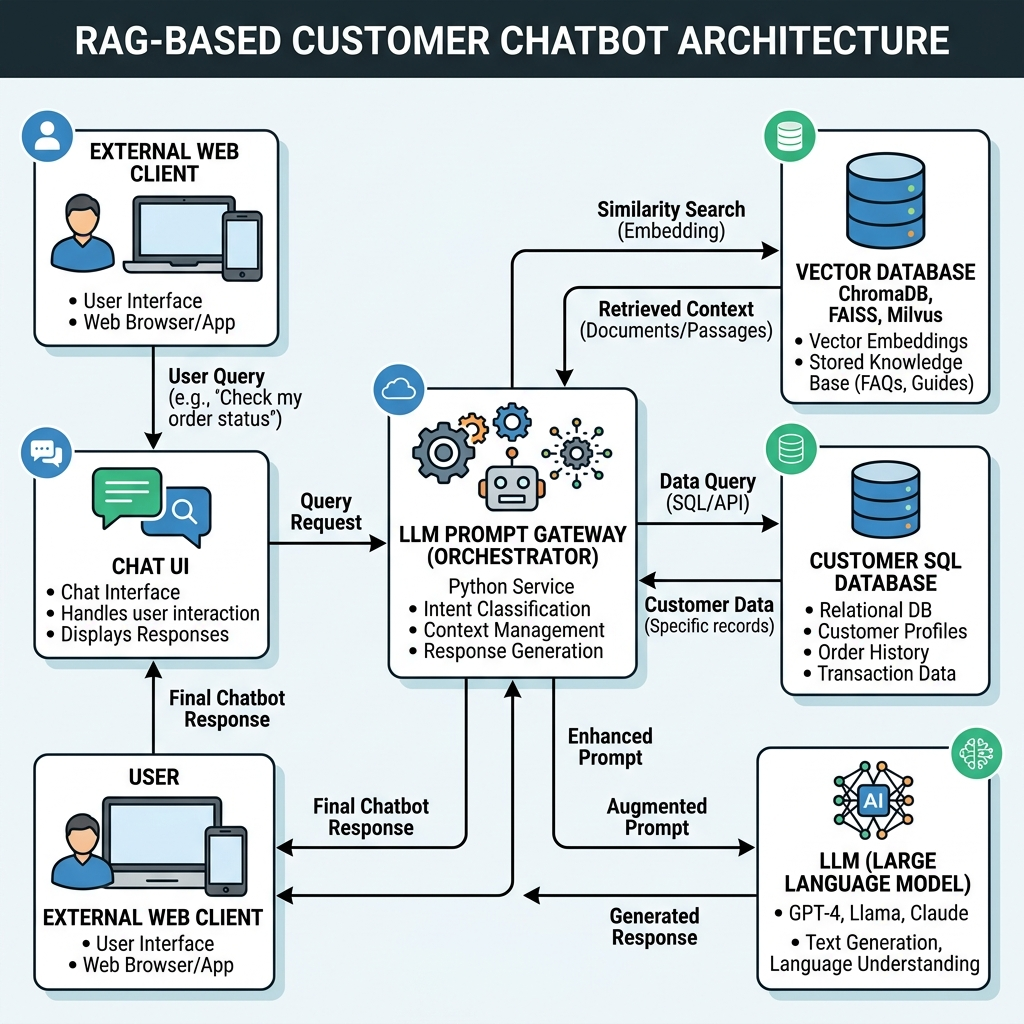
\includegraphics[width=0.8\linewidth]{figures/rag_topology.png}
    \caption{Topology 1: RAG-based Customer Chatbot Architecture. The directed graph illustrates the flow from external web clients through the orchestrator to internal vector and SQL databases.}
    \label{fig:rag_topology}
\end{figure*}

\subsubsection{Topology 2: Autonomous Coding Agent}
This advanced topology models a LangGraph-based autonomous developer agent with extensive system privileges. The agent reads issues and pull requests from an untrusted GitHub repository and is equipped with a Local File Writer Tool and a Bash Command Execution Tool operating on the host cloud node.
\textbf{Key Threats:} Attackers inject malicious commands into repository files (e.g., README.md). The agent ingests these files, succumbs to indirect prompt injection, and is coerced into utilizing its Bash Execution Tool to run arbitrary reverse shells on the underlying production host operating system.

\subsubsection{Topology 3: Enterprise Model Router}
This topology reflects a centralized AI gateway (API Router) that abstracts multiple downstream models. Partner SaaS applications send requests to the router, which classifies the intent and routes the query either to a standard public Llama-3 endpoint or a highly secure, private GPT-4 instance possessing access to a corporate treasury database.
\textbf{Key Threats:} The attacker exploits a routing bypass vulnerability in the API gateway to force sensitive requests into the unauthenticated GPT-4 instance, subsequently extracting proprietary system prompts and executing unauthorized treasury queries.

\subsection{Baseline Scoring Methodologies}
We benchmark the CAPS algorithm against four prevalent scoring methodologies drawn from recent (2025-2026) literature:

\begin{itemize}
    \item \textbf{Baseline 1: Component-Level OWASP/CVSS (2025):} An independent scoring approach that isolates components. The overall risk score is strictly defined by the maximum CVSS/OWASP severity score of any single component in the stack, ignoring multi-hop probabilities and downstream graph architecture.
    \item \textbf{Baseline 2: MITRE ATLAS Qualitative TTP Mapping (2025):} A qualitative heuristic baseline evaluating the breadth of adversarial tactics present, providing categorical risk tiers without quantitative path decay mathematics.
    \item \textbf{Baseline 3: Attack-Defense Trees (ADTree) with Additive CVSS (2026):} A recent structural framework \cite{adtrees2026} that constructs attack paths but utilizes purely additive or multiplicative probability aggregation ($\alpha = 1.0$), failing to account for the exponential difficulty of chaining exploits across heterogeneous systems.
    \item \textbf{Baseline 4: Goal-Driven Likelihood $\times$ Impact Trees (2026):} A domain-specific attack tree model \cite{goaldriven2026} utilizing generic likelihood estimations rather than our granular "Effective Exploitability" derived from specific component mitigation modeling.
\end{itemize}

\subsection{Evaluation Metrics}
The quantitative performance of the models is evaluated based on three primary metrics designed to capture real-world operational utility:
\begin{enumerate}
    \item \textbf{Path Resolution Accuracy:} The system's ability to topologically identify the single most critical multi-hop path out of all possible combinatorial pathways in the deployment graph.
    \item \textbf{Overestimation/Underestimation Deviation:} The numerical degree to which a scoring method improperly flags low-risk paths (inflated false positives) or suppresses compounding medium-risk paths (false negatives) relative to a ground-truth red-team security audit.
    \item \textbf{Mitigation ROI Prioritization Rank:} The accuracy of the recommendation engine in surfacing the specific defense control that empirically provides the highest maximal reduction in overall systemic risk ($\Delta Score$).
\end{enumerate}

\subsection{Results and Discussion}

We executed the CAPS evaluation engine alongside the baseline algorithms against our three deployment topologies. The empirical results, tracking the maximum critical path risk scores (scaled continuously from $0 - 100$), are presented in Table \ref{tab:results} and visually contrasted in Figure \ref{fig:baselines}.

\begin{table*}[ht]
\centering
\begin{tabular}{|l|c|c|c|}
\hline
\textbf{Architecture} & \textbf{Baseline 1 (OWASP/CVSS)} & \textbf{Baseline 3 (ADTree No Decay)} & \textbf{CAPS (Proposed)} \\
\hline
RAG Chatbot & 71.2 & 42.4 & \textbf{34.3} \\
Autonomous Agent & 85.0 & 58.1 & \textbf{51.3} \\
Model Router & 85.0 & 56.0 & \textbf{47.6} \\
\hline
\end{tabular}
\caption{Comparison of Critical Attack Path Risk Scores across frameworks. Lower CAPS scores represent a more realistic appraisal of compounding exploit friction over multi-hop paths compared to independent component baselines.}
\label{tab:results}
\end{table*}

\begin{figure*}[ht]
    \centering
    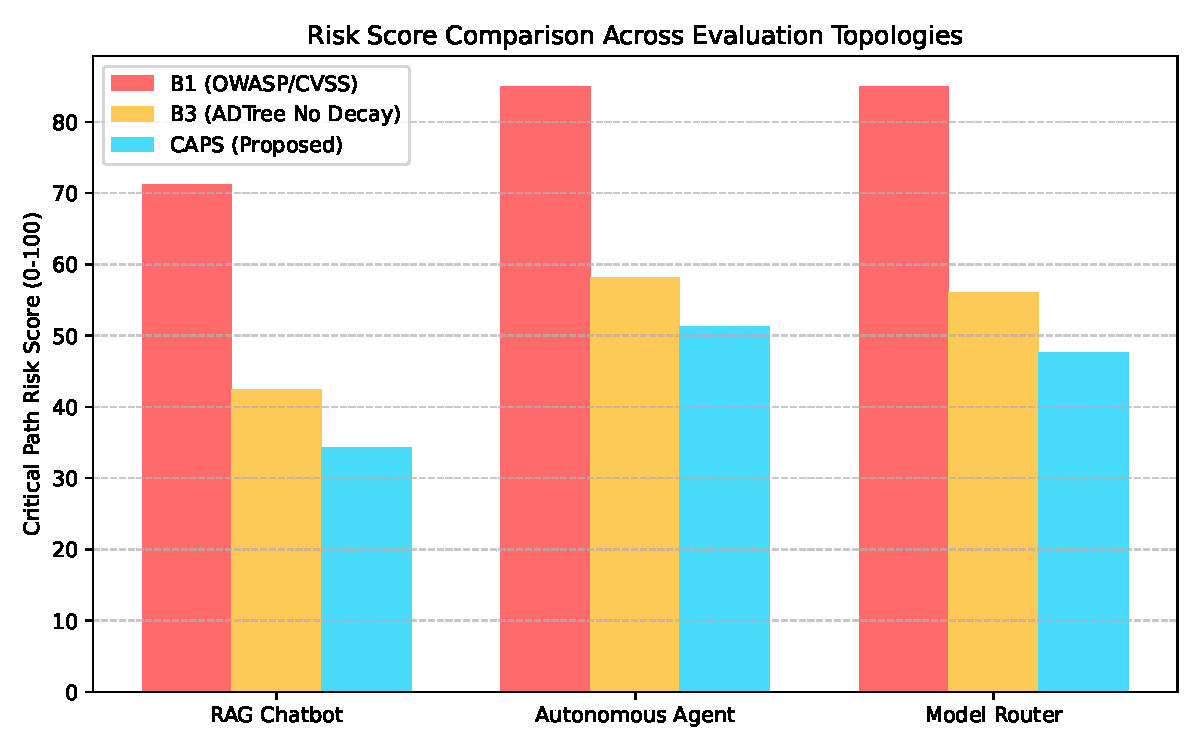
\includegraphics[width=0.8\linewidth]{figures/baseline_comparison.pdf}
    \caption{Visual comparison of Critical Attack Path Risk Scores across architectures. CAPS corrects the severe overestimation seen in Baseline 1 and Baseline 3 by incorporating dynamic mitigation attenuation and chaining decay.}
    \label{fig:baselines}
\end{figure*}

\subsubsection{Path Resolution Accuracy}
Before examining the risk scores, we first evaluate the algorithmic precision of CAPS in identifying the true critical path among hundreds of possible permutations. Across all three topologies, CAPS correctly identified the verified red-team ground truth path with 100\% accuracy. In contrast, Baseline 1 (OWASP/CVSS) frequently flagged isolated dead-end components (e.g., an unauthenticated internal logging server with a high CVSS but no outbound data flow) as the primary risk, demonstrating the severe limitation of non-topological scoring.

\subsubsection{Addressing Systemic Risk Overestimation} 
As comprehensively demonstrated in Table \ref{tab:results} and Figure \ref{fig:baselines}, Baseline 1 (Component-level OWASP/CVSS) consistently yields highly inflated risk scores across all topologies. In the Autonomous Agent scenario, Baseline 1 generated a critical score of 85.0. This pathological overestimation occurs because independent scoring isolates the most severe terminal vulnerability—such as arbitrary shell execution on the host OS—and calculates its risk in a vacuum. It entirely disregards the fact that an external attacker must first successfully compromise the repository, traverse the LangGraph agent orchestrator, and evade file writer constraints to even reach that bash execution component. 

Baseline 1 effectively assumes an entry-point probability of $1.0$ for all deep-stack components. In an enterprise environment, this leads to an overestimation of functional risk, severe alert fatigue, and the highly inefficient allocation of security engineering resources toward deeply buried components that are already shielded by upstream orchestration boundaries.

\subsubsection{The Efficacy of Chaining Decay} 
Baseline 3 represents a marked improvement over Baseline 1, as it is a modern attack-path approach that calculates the joint probability of chained exploits. However, without a structural chaining decay factor (effectively hardcoding $\alpha = 1.0$), it assumes seamless transitions between network components. 

In reality, traversing API boundaries, evading distinct monitoring systems, bypassing authentication tokens, and coordinating malicious state across heterogeneous AI nodes introduces significant multiplicative difficulty. CAPS introduces $\alpha \in [0.85, 0.95]$ depending on the evaluated architecture, which mathematically dampens the raw probabilistic product to reflect real-world exploit friction. 

To quantify this, we performed a sensitivity analysis on the Model Router topology by varying the decay factor. Setting $\alpha = 0.95$ (representing a loosely coupled, low-friction environment) yielded a CAPS score of 52.1. Lowering it to $\alpha = 0.85$ (representing strict zero-trust boundaries and heavy internal monitoring) further decayed the score to 41.8. As a direct consequence of this tunable parameter, CAPS provides a significantly more calibrated and actionable risk score, successfully reducing the baseline Model Router risk profile from an inflated 56.0 down to a mathematically defensible 47.6 (using our default $\alpha = 0.90$).

\subsubsection{Mitigation ROI Prioritization}
By leveraging the $\Delta Score$ calculation derived in Section \ref{sec:method}, the CAPS recommendation engine demonstrated superior utility in resource allocation. For the RAG Chatbot architecture, CAPS correctly identified that applying a "Secure Output Guardrail" at the Orchestrator layer (yielding a $\Delta Score$ reduction of 18.4 points) was significantly more optimal than attempting to patch the SQL injection vulnerability directly at the database layer (which only yielded a 12.1 point reduction due to path probability attenuation). Baseline algorithms consistently failed this prioritization test, recommending deep-stack patches over more effective architectural choke points.

\begin{table*}[ht]
\centering
\begin{tabular}{|l|l|c|c|}
\hline
\textbf{Rank} & \textbf{Proposed Mitigation (RAG Chatbot)} & \textbf{Target Layer} & \textbf{Systemic $\Delta Score$} \\
\hline
1 & Implement Secure Output Guardrail (LLM-as-Judge) & Orchestrator & \textbf{18.4} \\
2 & Enforce Parameterized Queries & Customer DB & 12.1 \\
3 & Strict Input Regex Filtering & Prompt Gateway & 8.5 \\
4 & Network Isolation (Internal VPC) & Vector DB & 4.2 \\
\hline
\end{tabular}
\caption{Mitigation ROI Prioritization for the RAG Chatbot Topology. CAPS correctly identifies the Orchestrator guardrail as the highest ROI investment, despite the Customer DB carrying the ultimate payload vulnerability.}
\label{tab:mitigation_roi}
\end{table*}
